% !TeX root = ../tfg.tex
% !TeX encoding = utf8
%
%*******************************************************
% Capítulo 8. Materiales y métodos
%*******************************************************

\chapter{Materiales y métodos}\label{cap:materiales}

\section{Conjunto de datos ID}\label{sec:conjunto-id}

El punto de partida se trata de una base de datos de imágenes médicas clasificadas según el tipo de enfermedad que presentaban. La base contaba con las siguientes clases: \clase{Adenocarcinoma\_ductal}, \clase{Glandulas\_no\_neoplasicas}, \clase{Gleason\_4\_fusionadas}, \clase{Gleason\_5\_comedonecrosis}, \clase{No\_Cancer}, \clase{Carcinoma\_intraductal}, \clase{Gleason\_3}, \clase{Gleason\_4\_glomeruloide}, \clase{Gleason\_5\_no\_glandulas}, \clase{PIN\_de\_alto\_grado}, \clase{Estroma}, \clase{Gleason\_4\_cribiformes}, \clase{Gleason\_4\_pobremente\_formadas} e \clase{Inflamatorio}.

La información de este apartado procede del artículo del conjunto de datos~\cite{ayensa2026}. El muestreo tisular fue realizado por patólogos experimentados con un amplio conocimiento en hispatología del cancer de próstata.
En definitiva nuestro conjunto de datos consiste en muestras de prostatectomía radical, durante su obtención las piezas se procesaron en un procesador automático de tejidos, se deshidrataron y se incluyeron en parafina. Se obtuvieron cortes de 3--5\,\si{\micro\metre} de grosor con un micrótomo, que se montaron en portaobjetos de vidrio, se desparafinaron y se tiñeron con hematoxilina y eosina (H\&E).

Las preparaciones teñidas con H\&E se digitalizaron con un escáner de preparaciones completas Aperio/Leica AT2 a 20$\times$ aumentos, con una resolución de escaneo de \num{50000} píxeles por pulgada (0,5\,\si{\micro\metre}/píxel). Las anotaciones se realizaron sobre 85 de esas imágenes de lámina completa (WSI).  Al igual que en el muestreo tisular todas las imágenes fueron segmentadas manualmente por patólogos experimentados con un amplio conocimiento de la histología del cáncer de próstata. Las regiones anotadas se clasificaron en 14 categorías histológicas distintas que reflejan patrones morfológicos reconocidos en la práctica clínica.

Cada WSI anotada se dividió en parches cuadrados de tamaño $H \times H = 224 \times 224$ píxeles, y para evitar continuaciones directas entre una imagen y otra
se aplicó un paso (\emph{stride}) de $p = 256$ píxeles. Un parche se asignaba a una clase concreta si más del 75\,\% de sus píxeles pertenecían a una región anotada como dicha clase; en caso contrario, se descartaba.


Respecto a las clases aparece cierto grado de confusión entre las siguientes casos. Estas similitudes han sido halladas mediante el análisis de las matrices de confusión de los 5 modelos, considerando que únicamente existe una confusión real entre clases cuando todos los modelos la presentan. Además como referencia se usará los datos de la matriz de confusión de swin\_small\_patch4\_window7\_224 que se pueden observar en la figura 9.10:
\begin{itemize}
  \item \textbf{Gleason 3, glándulas no neoplásicas y glándulas 4 fusionadas:} Dado el conjunto de imágenes de Gleason 3 un 8,6\%  es clasificado como glándula no neoplásica y 4,7\% como Gleason 4 fusionadas.
  \item \textbf{Gleason 4 fusionadas con Gleason 3 y Gleason 4 cribiformes:} Las imágenes son clasificadas como Gleason 3 en 1,6\% de los casos y en Gleason 4 cribiformes en un 4\%.
  \item \textbf{Glomeruloides con Gleason 4 cribiformes:} Las imágenes son clasificadas en la clase incorrecta en un 32\% de los casos y un acierto de 52 \%. Cabe destacar el caso del modelo efficientnetv2\_s el cual llega a tener una clasificacion incorrecta como cribiformes del 36\% y un acierto del 48\%.
  \item \textbf{Gleason 5 comedonecrosis con Gleason 4 cribiformes:} Este error de clasificacion es espcialmente particular, pues en aquellos casos en los que los modelos clasifican mal una muestra, esta solo es clasificada en la clase Gleason 4 cribiformes. Todos los modelos presentan un error similar, 14,28\% de clasificacion incorrecta frente al 85,7\% de acierto. El caso más grave lo presenta el modelo Resnet50 con 23,21\% en la clase equivocada nombrada y un 66,07\% de acierto.
\end{itemize}

Se ha consultado de forma auxiliar a un profesional del ámbito sanitario del hospital Virgen del Rocío (Sevilla) para tratar de entender a que se pueden deber estas confusiones. \revisar{Iván}
\begin{itemize}
  \item Como se ha visto antes, los modelos clasifican de forma erronea Gleason 3 como glandulas 4 fusionadas y viceversa. Esto se puede deber a que las muestras de Gleason 3 estan bien delimitadas y en Gleason 4 cribiformes hay una organización más anormal, según la partición que haga una clasificación Gleason 3 puede pertenecer a Gleason 4 cribiforme, de forma que se trata de una clasificación subjetiva.
  \item Tanto Gleason 5 comedonecrosis como Gleason 4 cribiformes son proliferacion tumorales de patrón cribiforme, por lo que mantienen una estructura similar lo único que difieren es en la necrósis central que presentan gleason 5 que puede ser dificil de determinar si ocupa superficie menor o si no aparece bien en el parche.
\end{itemize}
% En el preámbulo:
% \usepackage{booktabs}
% \usepackage{multirow}
% \usepackage{tabularx}
% \usepackage{array}

\begin{table}[htbp]
\centering
\footnotesize
\renewcommand{\arraystretch}{1.15}
\begin{tabularx}{\textwidth}{>{\raggedright\arraybackslash}p{2.6cm} >{\raggedright\arraybackslash}p{3.4cm} >{\raggedright\arraybackslash}X}
\toprule
\textbf{Categoría} & \textbf{Clase} & \textbf{Descripción} \\
\midrule
\multirow{4}{=}{Tejido no maligno}
 & Estroma (HS) & Tejido de sostén de la próstata; es músculo liso y tejido conjuntivo. \\
 & Glándulas no neoplásicas (NG) & Glándulas prostáticas normales. Son estructuras huecas con dos capas de células (basal y luminal). \\
 & Tejido sano no estromal & Tejido benigno que no pertenece a ninguna de las clases anteriores, como por ejemplo vasos sanguíneos o tejido adíposo. Se trata de una clase pequeña. \\
 & Tejido inflamatorio & Acúmulo de células inmunitarias; no se trata de cáncer y se identifica mediante muchos núcleos pequeños, oscuros, redondos y muy juntos. \\
\midrule
Gleason 3
 & Gleason 3 (G3) & Cáncer con glándulas bien formadas e individuales. Más pequeñas que las normales y se encuentran entre glándulas sanas. \\
\midrule
\multirow{4}{=}{Gleason 4}
 & Cribiformes (G4c) & Masa grande de células atravesada por muchas luces pequeñas, como un colador. \\
 & Fusionadas (G4f) & Glándulas que se han unido unas con otras sin estroma entre ellas, formando estructuras irregulares. \\
 & Pobremente formadas (G4p) & Debido a que en el campo de la medicina hay muchas escalas de grises, ciertas muestras no pueden ser clasificadas en ninguna clase en concreto por lo que se decide clasificar todas estas muestras independientes en una misma clase conjunta. Correspondería a una subclase de Gleason 4 caracterizadas por ser estructuras glandulares tumorales pequeñas, irregulares y mal definidas, con luces glandulares difíciles de identificar o prácticamente ausentes. Presentan una arquitectura incompleta que impide reconocer la formación de glándulas bien delimitadas, característica del patrón Gleason 3.\\
 & Glomeruloides (G4g) & Glándula dilatada con un ovillo de células dentro, unido a un lado de la pared. \\
\midrule
\multirow{2}{=}{Gleason 5}
 & Comedonecrosis (G5c) & Nidos sólidos o cribiformes de células tumorales con un centro de células muertas (necrosis), que se ve como un material rosado y sucio con restos de núcleos. \\
 & Sin glándulas & El tumor ya no forma glándulas. Aparecen láminas sólidas, cordones o células sueltas infiltrando el estroma. Es el patrón más agresivo. \\
\midrule
\multirow{3}{=}{Lesiones que no se gradúan con Gleason}
 & PIN de alto grado & Conductos y glándulas preexistentes (con su forma normal) revestidos por células con aspecto atípico (núcleos grandes, nucléolos visibles). \\
 & Carcinoma intraductal (IC) & Células malignas que rellenan y ensanchan los conductos existentes, formando patrones sólidos o cribiformes densos y con mucha más atipia que el PIN. \\
 & Adenocarcinoma ductal (DA)* & Una variante del cáncer de próstata que crece formando glándulas grandes revestidas por células altas y alargadas (cilíndricas), a menudo con estructuras papilares. \\
\bottomrule
\end{tabularx}
\caption{Explicación breve de cada clase.}
\label{tab:clases}
\vspace{2pt}
\begin{minipage}{\textwidth}
\footnotesize * DA presenta 13117 parches pero de solo 12 pacientes; esto refleja la alta probabilidad de que se entrene con parches de una misma lámina que también presente parches en test.
\end{minipage}
\end{table}

% La discrepancia con los nombres de fichero (identificación de las láminas y rejilla de 224 px) se trata en
% \cref{sec:fuga-laminas}.

% En el preámbulo:
% \usepackage{booktabs}
% \usepackage{multirow}
% \usepackage{tabularx}
% \usepackage{array}

\section{Partición e integridad}\label{sec:particion}

Inicialmente el repositorio cuenta con dos subcarpetas, \texttt{train} y \texttt{val}, con un total de \num{126109} imágenes (\num{113491} en \texttt{train} y \num{12618} en \texttt{val}), cuya distribución por clase se recoge en la \cref{tab:particion}.

% Generado por scripts/generar_tablas.py a partir de results_integridad/inventario_por_clase.csv. No editar a mano.
\begin{table}
\centering
\small
\caption{Número de imágenes por clase en la partición original del conjunto ID (carpetas \texttt{train} y \texttt{val}) y en la partición usada en este trabajo (el \texttt{train} original dividido 80/20 por clase en entrenamiento y validación; el \texttt{val} original como test).}
\label{tab:particion}
\begin{tabular}{lrrrrr}
\toprule
& \multicolumn{2}{c}{Original} & \multicolumn{3}{c}{Partición del TFG} \\
\cmidrule(lr){2-3}\cmidrule(lr){4-6}
Clase & Train & Val & Train & Validación & Test \\
\midrule
\clase{Adenocarcinoma\_ductal} & \num{18917} & \num{2102} & \num{15134} & \num{3783} & \num{2102} \\
\clase{Carcinoma\_intraductal} & \num{1083} & \num{121} & \num{867} & \num{216} & \num{121} \\
\clase{Estroma} & \num{22219} & \num{2469} & \num{17776} & \num{4443} & \num{2469} \\
\clase{Glandulas\_no\_neoplasicas} & \num{32304} & \num{3590} & \num{25844} & \num{6460} & \num{3590} \\
\clase{Gleason\_3} & \num{2275} & \num{253} & \num{1820} & \num{455} & \num{253} \\
\clase{Gleason\_4\_cribiformes} & \num{12723} & \num{1414} & \num{10179} & \num{2544} & \num{1414} \\
\clase{Gleason\_4\_fusionadas} & \num{6938} & \num{771} & \num{5551} & \num{1387} & \num{771} \\
\clase{Gleason\_4\_glomeruloide} & \num{218} & \num{25} & \num{175} & \num{43} & \num{25} \\
\clase{Gleason\_4\_pobremente\_formadas} & \num{1136} & \num{127} & \num{909} & \num{227} & \num{127} \\
\clase{Gleason\_5\_comedonecrosis} & \num{499} & \num{56} & \num{400} & \num{99} & \num{56} \\
\clase{Gleason\_5\_no\_glandulas} & \num{10908} & \num{1213} & \num{8727} & \num{2181} & \num{1213} \\
\clase{Inflamatorio} & \num{714} & \num{80} & \num{572} & \num{142} & \num{80} \\
\clase{No\_Cancer} & \num{1081} & \num{121} & \num{865} & \num{216} & \num{121} \\
\clase{PIN\_de\_alto\_grado} & \num{2476} & \num{276} & \num{1981} & \num{495} & \num{276} \\
\midrule
\textbf{Total} & \num{113491} & \num{12618} & \num{90800} & \num{22691} & \num{12618} \\
\bottomrule
\end{tabular}
\end{table}


El primer reto al que se enfrenta este trabajo es el de poder crear un modelo de aprendizaje supervisado que, dada una imagen de nuestro conjunto de datos, sea capaz de clasificarla en una de las respectivas clases con la mayor precisión posible.

Para comenzar se necesita un conjunto de entrenamiento, uno de validación y uno de test. Así pues, dada la estructura inicial del conjunto de datos, se optó por utilizar el directorio \texttt{val}, que presentaba una menor cantidad de imágenes en comparación con \texttt{train}, para realizar el test, y a su vez \texttt{train} se dividió de forma estratificada por clase, en proporción 80/20, en dos carpetas: una mayor para el entrenamiento y una menor para la validación. Se cuenta así con un total de \num{90800} imágenes para entrenamiento, \num{22691} para validación y \num{12618} para test. 
El reparto se hizo sin fijar una semilla aleatoria, por lo que no es reproducible. \revisar{Iván, ¿hace falta que ponga lo de la semilla?}

% Las notas incluían además una tabla resumen (Train ID 90.800, Validación ID 22.691, Test ID
% 12.618), recogida en la fila Total de la \cref{tab:particion}.


\subsection{Verificación de la integridad}\label{sec:integridad}

% Puntos que debería cubrir (results_integridad/resumen.md):
% - Inventario y md5 de los 252.218 ficheros (original y particiones del TFG).
% - El test es exactamente la carpeta val original y train \cup val es exactamente la carpeta train
%   original: mismos nombres, mismas carpetas de clase, contenido idéntico byte a byte.
% - Ningún duplicado exacto (md5) ni posición (lámina, x, y) repetida.
% - Las cifras por clase coinciden con la regla \lfloor 0,2 n \rfloor del script de partición
%   (p. ej., Adenocarcinoma_ductal: 18.917 \to val 3.783, train 15.134).
% - El script usa random.shuffle sin semilla y copia (no mueve) los ficheros.
% - La fuga por lámina de la partición original se trata en el \cref{cap:fuga}.
\pendiente{verificación de la integridad de la partición}

\section{Conjuntos OOD}\label{sec:conjuntos-ood}

\Cref{tab:diseno-ood} resume los conjuntos OOD empleados, el papel de cada uno y qué cambia respecto al conjunto ID.

\begin{table}[tbp]
  \centering
  \footnotesize
  \caption{Diseño de los conjuntos OOD: papel de cada conjunto, qué cambia respecto al conjunto ID y objetivo de su inclusión. Entre paréntesis, el número de imágenes.}
  \label{tab:diseno-ood}
  \begin{tabularx}{\textwidth}{@{}>{\raggedright\arraybackslash}p{0.2\textwidth}>{\raggedright\arraybackslash}p{0.12\textwidth}>{\raggedright\arraybackslash}X>{\raggedright\arraybackslash}X@{}}
    \toprule
    \textbf{Conjunto} & \textbf{Papel} & \textbf{¿Qué cambia respecto al ID?} & \textbf{Objetivo} \\
    \midrule
    (A) NCT-CRC: TUM + NORM (\num{23080}) & Near-OOD & Otro órgano (colon, tejido glandular) y otro centro; misma escala & Buscamos ver si es capaz de rechazar un tejido muy parecido al original \\
    (B) NCT-CRC: STR, LYM, MUS (por separado) & Control interno & Otro centro; tejidos parecidos a clases de entrenamiento (estroma e inflamatorio) & Tejidos nuevamente parecidos a ID: determinamos si descarta por el centro o por el tejido \\
    (C) PANDA (\num{10000})~\cite{bulten2022,kagglepanda128} & Cambio de centro y de escala & Mismo órgano (próstata), otros centros y escáneres; aumento mucho menor (cada tesela abarca una región de tejido mucho mayor) y más fondo blanco & Comprobar si el detector señala tejido del mismo órgano adquirido en condiciones muy distintas \\
    Control de resolución (\num{12618}) & Control & Las mismas imágenes del test ID, reducidas a 128\,px y ampliadas a 224\,px & Valorar únicamente el efecto de la pérdida de detalle (no reproduce la escala de PANDA) \\
    Corrupciones sintéticas (\num{12618} $\times$ 27) & \emph{Covariate shift} sintético & Las mismas imágenes del test ID con 9 corrupciones en 3 niveles de severidad & Comprobar si el detector señala artefactos de adquisición y si su puntuación gradúa la severidad \\
    DTD / \emph{Textures} & Far-OOD & No es tejido: texturas genéricas & Referencia sencilla: el detector debe señalarla como OOD \\
    NCT-CRC: ADI, BACK, DEB, MUC & Anexo (\cref{ap:anexo-nct}) & Grasa, fondo, restos, moco & \\
    \bottomrule
  \end{tabularx}
\end{table}
\revisar{fila «Corrupciones sintéticas» añadida por el agente (\cref{sec:corrupciones})}
\revisar{tabla de las notas: corregidas erratas y redacción mínima («si descarta por el centro o por el tejido», «discriminación», «órgano»)}

\subsection{NCT-CRC-HE-100K-NONORM}\label{sec:nct}

\begin{itemize}
  \item Este es un conjunto de \num{100000} parches no superpuestos de imágenes histológicas teñidas con hematoxilina y eosina (H\&E) de cáncer colorrectal humano (CRC) y tejido normal~\cite{kather2018,kather2019}.
  \item Todas las imágenes son de $224 \times 224$ píxeles (px) a 0,5 micras por píxel (MPP). Se utiliza la versión NONORM, generada a partir de los mismos datos originales pero sin normalización de color mediante el método de Macenko, para no introducir un cambio artificial en la distribución~\cite{macenko2009}.
  \item Las clases de tejido son: tejido adiposo (ADI), fondo (BACK), desechos (DEB), linfocitos (LYM), moco (MUC), músculo liso (MUS), mucosa normal del colon (NORM), estroma asociado al cáncer (STR) y epitelio de adenocarcinoma colorrectal (TUM).
  \item Estas imágenes se extrajeron manualmente de $N = 86$ portaobjetos de tejido de cáncer humano teñidos con H\&E, de muestras embebidas en parafina y fijadas en formalina (FFPE) del NCT Biobank (Centro Nacional de Enfermedades Tumorales, Heidelberg, Alemania) y del archivo de patología UMM (University Medical Center Mannheim, Mannheim, Alemania).
   Las muestras de tejido contenían portaobjetos tumorales primarios de CRC y tejido tumoral de metástasis hepáticas de CRC; las clases de tejido normal se aumentaron con regiones no tumorales de muestras de gastrectomía para aumentar la variabilidad. Es el parecido en la metodología del proceso de obtención de muestras lo que ha determinado que este conjunto de datos haya sido usado en esta fase de experimentación.
\end{itemize}

El control interno consiste en evaluar el detector con distintas clases de un mismo conjunto de datos, NCT-CRC-HE-100K~\cite{kather2019}. Todas sus imágenes proceden del mismo centro y presentan, por tanto, el mismo \emph{covariate shift} respecto a los datos ID. Las clases utilizadas en nuestra experimentación son TUM (epitelio de adenocarcinoma colorrectal), 
NORM (mucosa colónica normal), STR (estroma asociado al cáncer, que cabría esperar que se parezca a la clase ID de estroma, HS), LYM (linfocitos, que cabría esperar que se parezcan 
a la clase ID Inflamatorio) y MUS (músculo liso, que también podría parecerse al estroma ID, ya que el estroma prostático contiene músculo liso). Si el detector rechaza las imágenes de STR, LYM y MUS con la misma capacidad que las de TUM y NORM, aunque se parezcan más a las clases ID, esto indicaría
que presenta cierta sensibilidad al \emph{covariate shift}, no podemos argumentar más allá de una mera suposición porque todas las imágenes presentan también \emph{semantic shift}, a pesar de que algunos puedan ser más cercanas al conjunto $ID$. Las imágenes de PANDA son del mismo órgano, pero proceden de otros centros, y se adquirieron a una escala muy distinta, por lo que combinan varios cambios respecto a los datos ID; el control de imágenes ID a 128\,px permite valorar únicamente 
el efecto de la pérdida de detalle. Por último, el conjunto Textures (DTD) sirve como referencia de que el detector funciona correctamente, ya que son las muestras que presentan una mayor diferencia con lo aprendido por el modelo.


\revisar{Iván, como consideras añadir aquí un par de imágenes LYM y de ID de esntroma para ver le parecido mencionado}
\subsection{PANDA}\label{sec:panda}

\textbf{PANDA (próstata de otros centros).} Biopsias del mismo órgano (próstata) y mismo tipo de tinción, pero de escáneres y hospitales distintos (Karolinska Institute / Radboud University)~\cite{bulten2022}. Se utilizan \num{10000} teselas de $128 \times 128$\,px del conjunto público preparado por iafoss~\cite{kagglepanda128}. En él, cada biopsia se lee en el nivel de menor resolución de la imagen original, se divide en teselas de $128 \times 128$\,px y se conservan las 16 con más tejido, es decir, las de menor suma de intensidades. A esta escala, cada tesela abarca una región de tejido mucho mayor que un parche ID (en ella caben decenas de glándulas). Si una biopsia no llega a 16 teselas, se completan con teselas blancas, lo que explica las 291 teselas sin tejido presentes en el conjunto. Para su evaluación, las teselas se reescalan a 224\,px.

De las \num{168256} teselas del conjunto (\num{10516} biopsias con 16 teselas cada una), se seleccionaron al azar \num{10000} (muestreo uniforme sin reemplazo, sin semilla fija), procedentes de \num{6568} biopsias distintas (entre 1 y 6 teselas por biopsia; mediana 1).

\subsection{Control de resolución y DTD}\label{sec:control-dtd}

% Puntos que debería cubrir:
% - Control de resolución: las 12.618 imágenes del test ID reducidas a 128 px y ampliadas a 224 px;
%   mismas etiquetas que el test ID. Exactitud del Swin-S en el control: 0,9077.
% - DTD (Cimpoi et al., 2014): 47 categorías de texturas \pendiente{comprobar}; número de imágenes
%   usadas.
\pendiente{control de resolución y DTD~\cite{cimpoi2014}}

\subsection{Corrupciones sintéticas}\label{sec:corrupciones}

% Puntos (cifras de OpenOOD/results_corrupciones: decisiones.md, resumen.md, comprobacion_*):
% 1. Motivación: PANDA combina cambio de centro, de escala y de fondo y no aísla cada efecto;
%    aquí, covariate shift controlado y graduable sobre las mismas imágenes del test ID
%    (\cref{def:covariate-shift}).
% 2. Papel: covariate shift sintético, no near-OOD; la etiqueta no cambia, solo P(X). En la
%    detección del espectro completo (\cref{def:deteccionfullspectrum}) serían csID; aquí se mide
%    si los detectores las señalan, con criterio clínico: rechazar lo que el clasificador puede
%    clasificar mal.
% 3. Generador: Zhang et al. (MICCAI 2022), github.com/superjamessyx/robustness_benchmark,
%    commit 2b288c11f944192bea7ffae912687d27b3ad220f (1-7-2022), sin fichero de licencia.
%    9 corrupciones, 5 niveles; se usan 1, 3 y 5: 27 celdas + limpia (nivel 0).
%    Antecedente en próstata: Schömig-Markiefka et al. (2021).
% 4. Parámetros por corrupción y nivel: \cref{tab:corrupciones}.
% 5. Aplicación: 12.618 PNG RGB de 224 px del test ID, uint8, antes del Resize y de la
%    normalización de ImageNet; después, el mismo flujo de inferencia. Solo motion_blur es
%    aleatoria (ángulo U(-45°, 45°)); semilla = 4 primeros bytes de
%    sha256("<fichero>|<corrupción>|<nivel>"); 23/23 regeneraciones idénticas bit a bit (MD5;
%    20 al azar + 3 de movimiento). Marcas y burbujas: el código usa los recursos de 96 px; se
%    usaron los de 224 px del propio repositorio sin modificar el código. hue: marcada en el código
%    como "unreliable and needs debug". Ninguna corrupción sustituida.
% 6. Exclusiones: sin transformaciones geométricas (orientación arbitraria; volteo y rotación en
%    el entrenamiento). Brillo y contraste en aug_transforms de fastai (±0,2, p = 0,75); el brillo
%    se mantiene como control.
% 7. Diseño pareado: ID = limpias, OOD = sus versiones corruptas en cada celda; referencias de los
%    detectores = las del resto del cap. 10 (train limpio), sin reajuste.
% 8. Métricas: exactitud por celda; AUROC y FPR@95 por celda con IC 95 % por bootstrap pareado por
%    imagen (1.000 réplicas, semilla 0); CEC; % de saturación de STOOD-X (K = 500; no se repitió con
%    K = 144, \cref{sec:stoodx-seleccion-k}); Spearman entre la caída de
%    exactitud y el AUROC sobre las 27 celdas.
% 9. Muestra: test completo; la regla de recursos (<= 6 h) daba una submuestra estratificada de
%    3.000 (test completo estimado en ~14 h en CPU); cambio decidido por el autor antes de ver
%    resultados. Nivel 0 frente a lo congelado: predicciones idénticas 100 % (0 distintas),
%    Spearman mínimo 0,99999983 en los 15 detectores, exactitud 0,96870 (igual a la congelada).

La evaluación con PANDA (\cref{sec:panda}) combina un cambio de centro, de escala y de fondo, por lo que no permite aislar el efecto de cada uno. Para estudiar un \emph{covariate shift} (\cref{def:covariate-shift}) controlado y graduable se aplican corrupciones sintéticas a las mismas imágenes del test ID. La etiqueta de cada imagen no cambia; solo cambia $P(X)$. Por eso este conjunto no es near-OOD, sino un \emph{covariate shift} sintético: en la detección del espectro completo (\cref{def:deteccionfullspectrum}) estas imágenes se aceptarían como csID. Aquí se evalúa si los detectores las señalan con un criterio clínico: rechazar aquello que el clasificador puede clasificar mal. \pendiente{justificación del autor}

Las corrupciones son las del banco de pruebas de Zhang et al.~\cite{zhang2022corruptions}, con su código público (commit \texttt{2b288c1}; el repositorio no tiene licencia). Son nueve corrupciones habituales en patología digital (brillo, saturación, tono, marcas, burbujas, compresión JPEG, pixelado, desenfoque y desenfoque por movimiento), cada una con cinco niveles de severidad, de los que se usan los niveles 1, 3 y 5 (\cref{fig:ejemplo-corrupciones,tab:corrupciones}): 27 celdas, más la imagen limpia (nivel 0). En próstata, Schömig-Markiefka et al.~\cite{schomig2021} ya aplicaron un enfoque similar.
\begin{figure}[tbp]
  \centering
  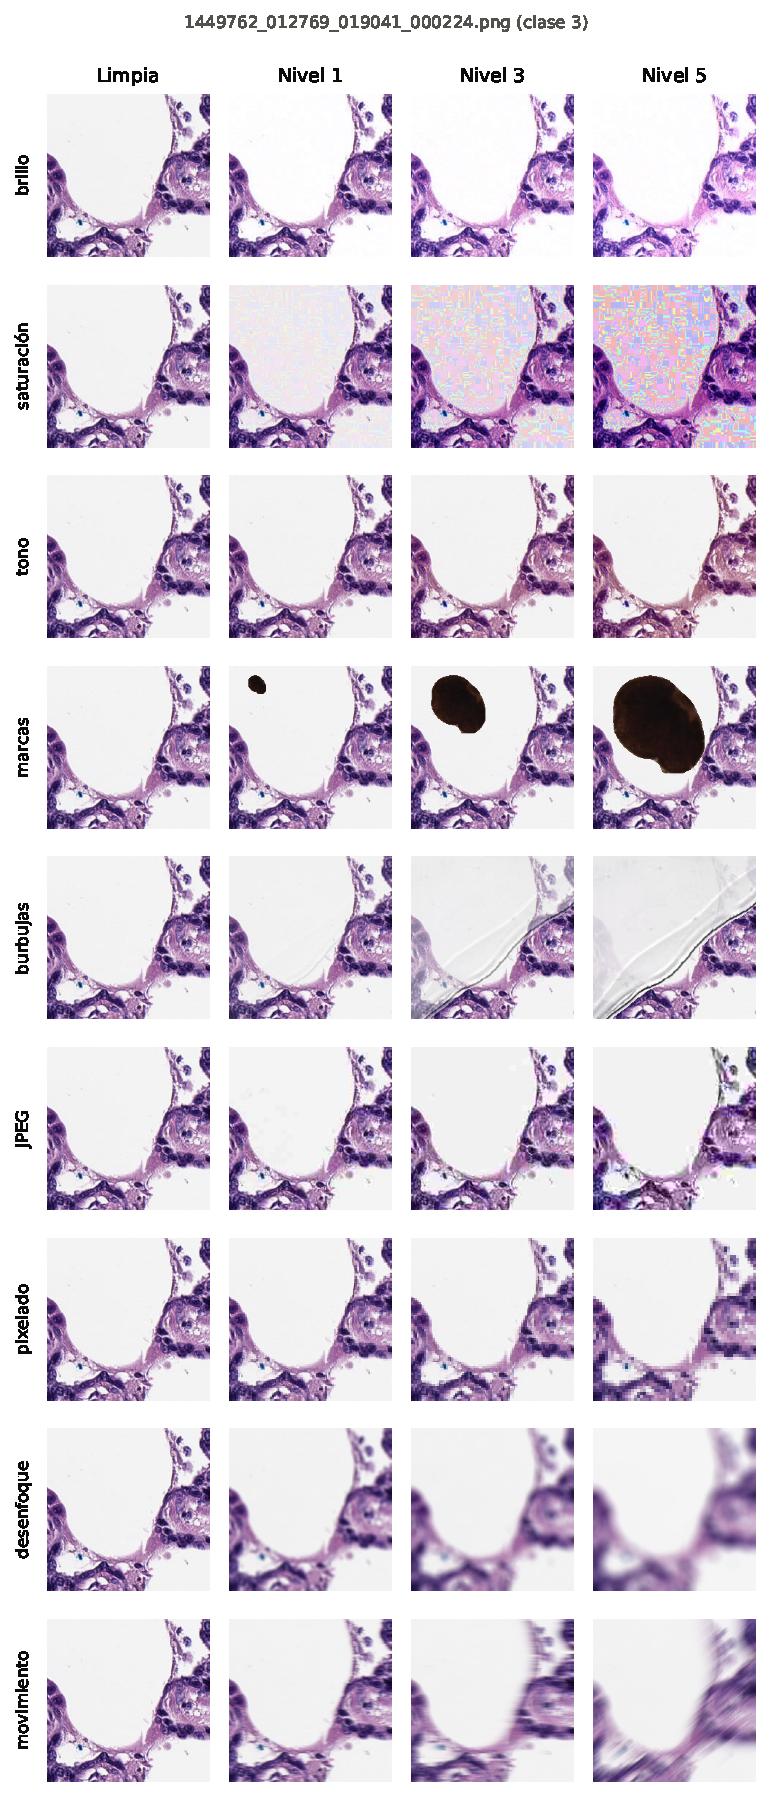
\includegraphics[width=\textwidth]{img/cap08/a_ejemplo_corrupciones.pdf}
  \caption{Ejemplo de las nueve corrupciones de Zhang et al.\ en los niveles de severidad 1, 3 y 5 sobre una imagen del test ID (clase \clase{Glandulas\_no\_neoplasicas}, imagen \texttt{1449762\_012769\_019041\_000224.png}). Fuente de las corrupciones: Zhang et al.~\cite{zhang2022corruptions}.}
  \label{fig:ejemplo-corrupciones}
\end{figure}
% Generado por scripts/generar_tablas.py a partir de results_corrupciones/parametros_corrupciones.csv. No editar a mano.
\begin{table}
\centering
\footnotesize
\setlength{\tabcolsep}{4pt}
\caption{Parámetros de las nueve corrupciones de Zhang et al.~\cite{zhang2022corruptions} en los niveles de severidad 1, 3 y 5. La severidad crece con el parámetro, salvo en JPEG y pixelado, en los que crece al bajar la calidad o el factor.}
\label{tab:corrupciones}
\begin{tabularx}{\textwidth}{@{}l>{\raggedright\arraybackslash}Xccc@{}}
\toprule
Corrupción & Parámetro & Nivel 1 & Nivel 3 & Nivel 5 \\
\midrule
Brillo & Incremento de V (HSV) & 0{,}05 & 0{,}15 & 0{,}25 \\
Saturación & Incremento de S (HSV) & 0{,}05 & 0{,}15 & 0{,}25 \\
Tono & Incremento de H (HSV, circular)$^{c}$ & 0{,}02 & 0{,}06 & 0{,}1 \\
Marcas & Tamaño de la mancha (alto $\times$ ancho)$^{a}$ & 26 $\times$ 24\,px & 80 $\times$ 75\,px & 135 $\times$ 126\,px \\
Burbujas & Proporción de mezcla con la burbuja$^{b}$ & 0{,}1 & 0{,}5 & 0{,}9 \\
JPEG & Calidad JPEG & 25 & 15 & 7 \\
Pixelado & Factor de reducción (filtro BOX) & 0{,}6 & 0{,}4 & 0{,}25 \\
Desenfoque & (radio del disco; $\sigma$ del antialias) & (3; 0{,}1) & (6; 0{,}5) & (10; 0{,}5) \\
Movimiento & (radio; $\sigma$) de ImageMagick; ángulo $\mathcal{U}(-45^\circ, 45^\circ)$ & (10; 3) & (15; 8) & (20; 15) \\
\bottomrule
\end{tabularx}

\smallskip
\parbox{\linewidth}{\scriptsize Marcas y burbujas usan los recursos de 224\,px del propio repositorio (el código usa por defecto los de 96\,px). Solo el desenfoque por movimiento es aleatorio: su semilla se deriva con SHA-256 del fichero, la corrupción y el nivel. $^{a}$Siempre la misma mancha, en la posición fija (27, 13). $^{b}$Se usa siempre la primera de las 6 burbujas del repositorio, en posición fija. $^{c}$Implementación marcada como poco fiable en el código original.}
\end{table}


Las corrupciones se aplican a las \num{12618} imágenes del test ID (PNG RGB de $224 \times 224$\,px) en píxeles \texttt{uint8}, antes del redimensionado y de la normalización de ImageNet; después se sigue el mismo flujo de inferencia que en el resto de conjuntos. Solo el desenfoque por movimiento es aleatorio. Su semilla se deriva de forma determinista del nombre del fichero, la corrupción y el nivel (SHA-256), de modo que cada imagen corrupta puede regenerarse: 23 de 23 regeneraciones fueron idénticas bit a bit. Para las marcas y las burbujas, el código usa por defecto recursos de 96\,px; se usaron los de 224\,px del propio repositorio, sin modificar el código. La implementación del tono está marcada en el propio código como poco fiable. No se sustituyó ninguna corrupción.

No se incluyen transformaciones geométricas: la orientación del tejido es arbitraria y el modelo se entrenó con volteo y rotación (\cref{sec:dataloader}). El brillo y el contraste formaban parte del aumento de datos del entrenamiento (\cref{sec:dataloader}; \texttt{aug\_transforms} de fastai~\cite{howard2020fastai}, $\pm 0{,}2$ con probabilidad $0{,}75$); el brillo se mantiene como control, ya que se espera que el modelo sea robusto a él.

El diseño es pareado: las imágenes limpias son las ID y sus versiones corruptas de cada celda, las OOD. Las referencias de los detectores son las mismas que en el resto del \cref{cap:deteccion-ood} (calculadas con el train limpio), sin reajustar nada. Así, el efecto de la corrupción queda aislado de cualquier diferencia de centro, escala o lámina. En cada celda se miden la exactitud del clasificador, el \AUROC (\cref{sec:auroc}) y el \FPRn{95} (\cref{sec:fpr95}), con intervalos de confianza del 95\,\% por \emph{bootstrap} pareado por imagen (\cref{sec:bootstrap}; \num{1000} réplicas, semilla 0). Además se calculan la CEC (\cref{sec:cec}), el porcentaje de imágenes con la puntuación de \stoodx saturada (\cref{obs:u-empates}) y la correlación de Spearman entre la caída de exactitud y el \AUROC sobre las 27 celdas (\cref{def:spearman}).

Se usó el test completo. La regla de recursos fijada de antemano daba una submuestra de \num{3000} imágenes, porque el test completo tardaba unas 14\,h en CPU; el cambio se decidió antes de ver ningún resultado. Con el nivel 0 se comprobó que el cálculo reproduce la evaluación del resto del capítulo: las predicciones coinciden al 100\,\%, la correlación de Spearman entre puntuaciones es al menos 0,9999998 en todos los detectores y la exactitud es la misma. \revisar{la exactitud del nivel 0 es 0,96870, igual a la de las \emph{features} congeladas de la evaluación OOD (0,9687 [0,9657; 0,9716] en exactitud\_celda.csv), pero no a la de results\_fase1 (0,9688 [0,9658; 0,9717]): no se da la cifra}

\revisar{fin del borrador del agente}

\section{Entorno de ejecución}\label{sec:entorno}
\revisar{Iván: Considero que no aporta nada añadir los entornos que he usado y las cosas que tengo
instalados en ellos porque cada poco suelen cambiar, entonces algo que igual he usado yo, para un par de meses deja de servir}
Vamos a usar el repositorio OpenOOD~\cite{openood} para continuar con nuestro análisis de resultados.
\revisar{el enlace a GitHub se sustituye por la cita; el enlace al cuaderno de Colab con la explicación de uso y su captura de pantalla no van a la memoria}

% Puntos que debería cubrir (cifras de los ficheros de configuración):
% - Hardware: entrenamiento en una NVIDIA TITAN Xp (resultados.txt de param4; 583,6 min de
%   entrenamiento del Swin-S); evaluación OOD en una NVIDIA GeForce RTX 2080 Ti + 8 CPU
%   (config.json de la fase A).
% - Software de la evaluación OOD: Python 3.9.25, PyTorch 2.8.0 (CUDA 12.8), timm 1.0.25,
%   NumPy 1.26.4, scikit-learn 1.6.1, pandas 1.5.3, OpenOOD (commit 3c35632).
% - Software del entrenamiento: fastai 2.7.19 y PyTorch 1.12.1 (entorno fastai_env; slurm-*.out).
% - Software de la explicabilidad: torch 2.8 y fastai 2.7.19 (entorno crp_env).
% - Corrupciones sintéticas (\cref{sec:corrupciones}; results_corrupciones/decisiones.md y resumen.md):
%   CPU de dionisio (Intel Xeon Silver 4216 a 2,10 GHz), 12 hilos, fp32, entorno fastai_env_ood.
%   Sin GPU: la TITAN Xp de atenea (sm_61) no la soporta torch 2.8.0+cu128. «El resto de GPU
%   estaban ocupadas» no consta en los ficheros: decisiones.md dice que atenea y hera pasaron a
%   DRAIN (14-11-2026) y que titan (Pascal) y hera (driver roto) ya estaban excluidas: comprobar. Cálculo: 13 h 25 min; MaxRSS ~ 10,6 GB. Wand 0.6.13 e ImageMagick
%   6.9.10-23 Q16, copiados en results_corrupciones/pydeps/.
% - Detección OOD con ConvNeXt-S (\cref{ap:convnext}; results_ood_convnext/resumen.md y decisiones.md): nodo zeus,
%   solo CPU (Intel Xeon Silver 4114 a 2,20 GHz), 12 hilos, fp32, entorno fastai_env_ood; trabajo SLURM 192107:
%   8 h 56 min (8 h 56 min 12 s); MaxRSS 6,2 GiB (6.480.436 KB). El Swin-S se evaluó en GPU.
%   Espacio principal M (results_ood_convnext/espacio_principal/decisiones.md y configuracion_convnext.csv):
%   trabajos 192990 (preparación, 2 min 21 s), 192991 (detectores, 26 min 12 s; MaxRSS 3,0 GiB) y 192992
%   (tablas, 7 min 40 s), en zeus, solo CPU, 12 hilos, fp32; total 36 min (36 min 13 s).
\pendiente{hardware y software}

\section{Protocolo de entrenamiento}\label{sec:protocolo}

\subsection{DataLoader}\label{sec:dataloader}
\textcolor{green}{
Para una primera aproximación del modelo se decididió crear un conjunto de imágenes menor a partir del original, el cual sirve para pruebas y para comprobar el funcionamiento correcto de los distintos modelos antes de pasar a entrenar con el conjunto de datos original. Este, al igual que el conjunto de datos original, cuenta con tres carpetas: inicialmente se seleccionaron 10 imágenes de cada carpeta de la estructura original del conjunto de datos para crear uno nuevo, pero con un número mucho más reducido de imágenes. Posteriormente se aplicó el mismo procedimiento de separar \texttt{train} en dos nuevas carpetas de \texttt{train} y \texttt{val}, y el \texttt{val} original pasó a ser test. Debido a esto, el resultado final ha sido una estructura de tres carpetas: \texttt{train} con 139 imágenes, \texttt{val} con 55 y test con 167.
Cada imagen se redimensiona a 224\,px (excepto ConvNeXt-S donde las imágenes tienen que ser de 256) con \texttt{Resize(224, method='squish')}, que la estira sin recortarla. Durante el entrenamiento se aplica aumento de datos por lotes con \texttt{aug\_transforms()} de fastai 2.7.19~\cite{howard2020fastai}, con sus valores por defecto: volteo horizontal con probabilidad 0,5 (sin volteo vertical); rotación de hasta $\pm 10^\circ$, ampliación entre 1,0 y 1,1 y deformación de perspectiva de magnitud máxima 0,2, con probabilidad 0,75; y variación de brillo y contraste de magnitud máxima 0,2, con probabilidad 0,75. Los huecos de las transformaciones geométricas se rellenan por reflexión y no hay recorte aleatorio. Al final se normaliza con la media y la desviación típica de ImageNet. No se aplican cambios de tono ni de saturación, así que el color solo varía en brillo y contraste.
}
\subsection{Learner}\label{sec:learner}

En cuanto al optimizador, se usa AdamW (Loshchilov y Hutter~\cite{loshchilov2019}), pues se trata de una versión mejorada del optimizador Adam (Kingma y Ba~\cite{kingma2014}) con la mejora añadida de que cuenta con \emph{weight decay} (\cref{sec:adamw}). En la implementación de fastai es cierto que el nombre asociado es el de Adam, pero es debido a una decisión de fastai de adoptar la versión mejorada del optimizador bajo el nombre de la original.

\textcolor{green}{
Debido a la complejidad del problema, no tardó en aparecer el error de memoria \emph{CUDA out of memory}. Para manejar este problema sin alterar la arquitectura del modelo \pendiente{sustituir por fuente académica} se optó por reducir el tamaño del lote a la mitad, pasando así de 128 imágenes por lote a 64. Las otras medidas tomadas fueron adaptar el \emph{learner} para trabajar con precisión de 16 bits~\cite{micikevicius2018}, ahorrando así memoria, liberar la caché de la memoria al iniciar la ejecución y, por último, reducir el número de \emph{workers} de 8 a 4, planteando la posibilidad de que la creación de hebras separadas para el tratamiento del problema pudiera estar influyendo en una mayor lentitud de ejecución del modelo.
}
Respecto al resto de configuraciones para el entrenamiento de optaron por las siguientes.
\begin{itemize}
  \item \textbf{Preprocesado:} Redimensionado al tamaño de entrada mediante \nolinkurl{method='squish'} ($224\text{ px}$; ConvNeXt-S a $256\text{ px}$), aumentación de datos con \nolinkurl{aug_transforms()} de fastai y normalización usando las estadísticas de ImageNet.
  \item \textbf{Función de pérdida:} \texttt{LabelSmoothing\allowbreak CrossEntropy} ($\varepsilon = 0{,}1$, \cref{def:label-smoothing}).
  \item \textbf{Optimizador (común a los cinco):} Adam de fastai con decaimiento desacoplado (AdamW) y \texttt{wd = 0.1}.
  \item \textbf{Gestión de memoria:} Tamaño de lote de $64$ y precisión mixta mediante \nolinkurl{to_fp16()}.
  \item \textbf{Parada temprana:} \texttt{EarlyStopping\allowbreak Callback} monitorizando \nolinkurl{valid_loss} (\nolinkurl{min_delta = 0.005}, \nolinkurl{patience = 10}).
  \item \textbf{ViT-B/16, ResNet-50, ConvNeXt-S y EfficientNetV2-S}: Instanciados con \nolinkurl{vision_learner} (\texttt{ps = 0.5}), búsqueda de tasa de aprendizaje con \nolinkurl{lr_find} (\textit{valley}) y entrenamiento mediante \nolinkurl{fine_tune} ($10$ épocas iniciales congeladas seguidas de hasta $90$ épocas descongeladas).
  \item \textbf{Swin-S}: Instanciado directamente con \texttt{Learner} sobre el modelo de \texttt{timm} y entrenado sin congelación previa mediante \nolinkurl{fit_one_cycle} ($25$ épocas, $\text{lr}_{\max} = 10^{-4}$).
\end{itemize}
\begin{quote}
\small \textbf{Justificación del protocolo de Swin-S:} A diferencia del resto de arquitecturas evaluadas ---entrenadas mediante el protocolo estándar \texttt{fine\_tune} en dos fases ($10$ épocas iniciales con el \textit{backbone} congelado para estabilizar la cabeza clasificadora y un posterior ajuste fino global)---, el modelo \textbf{Swin-S} se entrenó directamente de extremo a extremo mediante \texttt{fit\_one\_cycle} sin congelación previa. En arquitecturas basadas en \textit{Vision Transformers} jerárquicos, el bloqueo inicial de los bloques de autoatención puede limitar la adaptación conjunta de las representaciones globales a las particularidades del dominio; el calentamiento progresivo (\textit{warm-up}) propio de la política \textit{1cycle} resulta suficiente para amortiguar los gradientes iniciales sin degradar los pesos preentrenados.
\end{quote}

%\pendiente{explicar la diferencia de protocolo: Swin-S con \texttt{fit\_one\_cycle} sin congelar; los otros cuatro modelos con \texttt{fine\_tune}}

Llegados a este punto, solo queda probar con diversos modelos ya preentrenados, hacerles un ajuste fino (\emph{fine tuning}) y analizar cuál genera mejores resultados, que será por tanto con el que sigamos trabajando a lo largo del proyecto (\cref{cap:clasificacion-id}).

\endinput
